\section{Introduktion}\label{sec:intro}
Denne aktivitet omhandler fremgangsmåden til opstilling og måling af overføringsfunktionen for en Buck-konverters udgangsfilter. De målte resultater sammenlignes med de beregnede amplitude- og fase-plots. Der inkluderes også brug af MATLAB, med et program som læser data fra en fil, og derved kan generere et bodeplot. \\
\\
Målet med denne aktivtet er at få de studerende til at forstå overføringsfunktionen for en Buck-konverter. Aktiviteten er også med til at give de studerende øvelse i de forskellige MATLAB kommandoer samt den generelle brug. Denne aktivitet skal danne grundlag for aktivitet 2. 

\section{Teori}\label{sec:teori}
En overføringsfunktion er beskrevet ved: (mangler)\\
\\
For at danne et udtryk for en overføringsfunktion ved en bestemt model, bruges almindelig kredsløbsanalyse. Kredsløbsanalysen indebærer at danne ækvivalent for serielle og parallelle forbindelser.

\begin{figure}[h!]
	\centering
	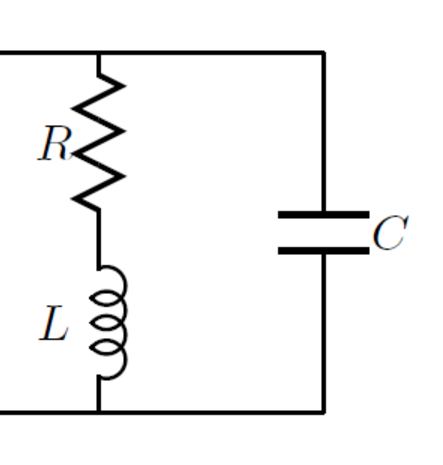
\includegraphics[width=.3\textwidth]{reg1/rlc.png}
	\caption{RLC-kredsløb}
	\label{fig:rlc}
\end{figure}